% Name: UML class diagram
% Description: Classes with attributes and methods, an association with multiplicities, and inheritance.
% Tags: UML, class diagram, inheritance, object-oriented

\usetikzlibrary{shapes.multipart, arrows.meta, positioning}

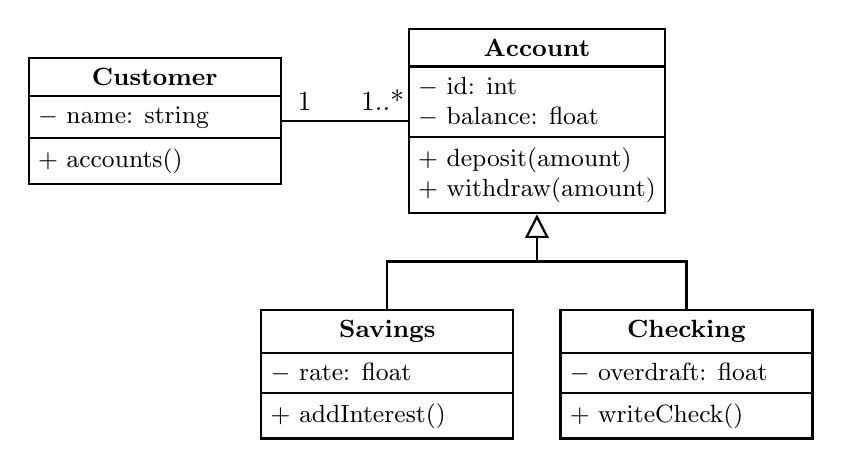
\begin{tikzpicture}[
  node distance=12mm and 16mm,
  class/.style={
    rectangle split, rectangle split parts=3, draw, thick, font=\small,
    rectangle split part align={center, left, left}, align=left, minimum width=32mm,
  },
  inherit/.style={-{Triangle[open, length=3mm, width=3mm]}, thick},
]
  \node[class] (account) {\textbf{Account}
    \nodepart{second} $-$ id: int \\ $-$ balance: float
    \nodepart{third} $+$ deposit(amount) \\ $+$ withdraw(amount)};
  \node[class, left=of account] (customer) {\textbf{Customer}
    \nodepart{second} $-$ name: string
    \nodepart{third} $+$ accounts()};
  \node[class, below=of account, xshift=-19mm] (savings) {\textbf{Savings}
    \nodepart{second} $-$ rate: float
    \nodepart{third} $+$ addInterest()};
  \node[class, below=of account, xshift=19mm] (checking) {\textbf{Checking}
    \nodepart{second} $-$ overdraft: float
    \nodepart{third} $+$ writeCheck()};

  \coordinate (join) at ([yshift=-6mm]account.south);
  \draw[thick] (savings.north) |- (join) -| (checking.north);
  \draw[inherit] (join) -- (account.south);
  \draw[thick] (customer) -- node[above, pos=0.18] {1} node[above, pos=0.8] {1..*} (account);
\end{tikzpicture}
